\documentclass[landscape]{foils}
\usepackage{graphicx}
\usepackage{amsmath}
\usepackage{hyperref}
\input defs.tex
\raggedright
\special{! TeXDict begin /landplus90{true}store end }
\renewcommand{\oursection}[1]{
\foilhead[-1.0cm]{#1}
}

\title{Objective-first optimization for nanophotonics}
\author{}
\MyLogo{Jesse Lu, Jelena Vuckovic group, Stanford University}
\date{}

\begin{document}
\setlength{\parskip}{0cm}
\maketitle

\BIT \itemsep -1pt
\item adjoint method
\item objective-first approach
\item field constraints: boundary-value problem
\item structure constraints: level-set formulation
\item example
\item ongoing and future work
\EIT

\vfill

\oursection{Adjoint method}
Typical formulation of a structural optimization problem:
\begin{align}
\mbox{decrease} & \quad f(x) \\
\subjectto & \quad g(x,p) = 0
\end{align}
\BIT
\item $f(x): \comps^n \to \reals$ is the \emph{design objective}
\item $g(x,p): \comps^n \times \reals^n \to \comps^n$ is the \emph{governing physics}
\item $x \in \comps^n$ is the field 
\item $p \in \reals^n$ is the structure 
\item $x$ is the dependent variable, $p$ is the independent variable
\EIT
\newpage

\BIT
\item problem is generally non-convex, so we optimize using only the first-order approximations,
\begin{align}
f(x_0+dx) & \approx f(x_0) + \pf{f}{x} dx \\
g(x_0+dx,p_0+dp) & \approx g(x_0,p_0) + \pf{g}{x} dx + \pf{g}{p} dp
\end{align}
\item assuming that $g(x_0,p_0) = 0$, the equality constraint is satisfied via
    \BEQ  dx = -\left(\pf{g}{x}\right)^{-1} \pf{g}{p} dp \EEQ
\EIT
\newpage

\BIT
\item now we can decrease $f(x_0+dx)$,
    \begin{align} 
    f(x_0+dx) & \approx f(x_0) + \pf{f}{x} dx \\
        & \approx f(x_0) - \pf{f}{x} \left(\pf{g}{x}\right)^{-1} \pf{g}{p} dp \\
        & \approx f(x_0) + \pf{f}{p} dp
    \end{align}
    by choosing $dp$ in the direction of $dp \propto -\pf{f}{p}$
\item computing $\pf{f}{p}$ can be reduced to a single field solve (\ie solving $g(x,p)$ for $x$, given $p$)
\EIT
\newpage

Characteristics of the adjoint method:
\BIT
\item can use existing field solvers 
\item each iteration requires two solves, one to calculate $\pf{f}{p}$, and the other to calculate the new $x$
\item need good initial guess, since this heavily influences what the final structure will be
\item optimization generally ``stalls'' on local minima
\EIT

\oursection{Objective-first approach}
ob-1 means that we prioritize the design objective over satisfying physics
\begin{align}
\mbox{decrease} & \quad \|g(x,p)\|^2 \\
\subjectto & \quad f(x) = 0
\end{align}
\BIT
\item $r(x,p) = \|g(x,p)\|^2$ is the \emph{physics residual}
\item $x$ always satisfies our design objective, we change $x$ and $p$ only to increasingly satisfy physics
\item $x$ and $p$ are both independent variables
\EIT
\newpage

\BIT
\item this problem is still non-convex, use linear approximation 
\begin{align}
r(x_0+dx,p_0+dp) & \approx r(x_0,p_0) + \pf{r}{x} dx + \pf{r}{p} dp \\
f(x_0+dx) & \approx f(x_0) + \pf{f}{x} dx 
\end{align}
\item decrease $r$ by choosing $dp \propto -\pf{r}{p}$
\item decrease $r$ by choosing 
    $dx \propto - (I - P_{f_x}) \pf{r}{x}$
\item $P_{f_x}$ is the projector onto the vector space defined by $\pf{f}{x}$, this satisfies the equality constraint
\item computing $P_{f_x}$ requires solving for $\left(\pf{f}{x}^T \pf{f}{x}\right)^{-1}$, but this is often \emph{trivial}
\EIT
\newpage


ob-1 requires only matrix multiplication (and trivial matrix solve)
\BIT
\item For 3D structures, most field solvers are based on (often $>10,000$) matrix multiplies
\item this means that is may be possible to solve larger design problems in the same amount of time needed for a field solve
\EIT

\vspace{3ex}

ob-1 should be less dependent on starting guess 
\BIT
\item some previous problems (using a similar approach) did not depend at all on initial structure
\item such a formulation may result in fewer local minima to stall on
\EIT
\vfill

\oursection{Field constraints: boundary-value problem}
\BIT
\item formulation of the constraint is the key issue
\item a sufficient constraint for most devices is to match field values along the border
\BEQ f(x) = \| x^\text{border} - x^\text{border}_0 \|^2 = 0 \EEQ
\item physics residual is the error in Maxwell's sourceless, time-harmonic equations
\BEQ \|g(x,p)\|^2 = \|A(p)x\|^2 = 
    \left\| \left[ 
    \begin{array}{cc}
        \nabla\times & i\mu\omega \\
        -ip\omega & \nabla\times
    \end{array}
    \right] 
    \left[ \begin{array}{c} x_E \\ x_H \end{array} \right] 
    \right\|^2
\EEQ
\item here $p$ determines the values of $\epsilon$
\EIT
\newpage

\BIT
\item to experiment, we fix $p = p_0$, which convexifies the ob-1 formulation
\begin{align}
\mbox{minimize} & \quad \|A(p_0)x\|^2 \\
\subjectto & \quad x^\text{border} = x^\text{border}_0
\end{align}
\begin{center}
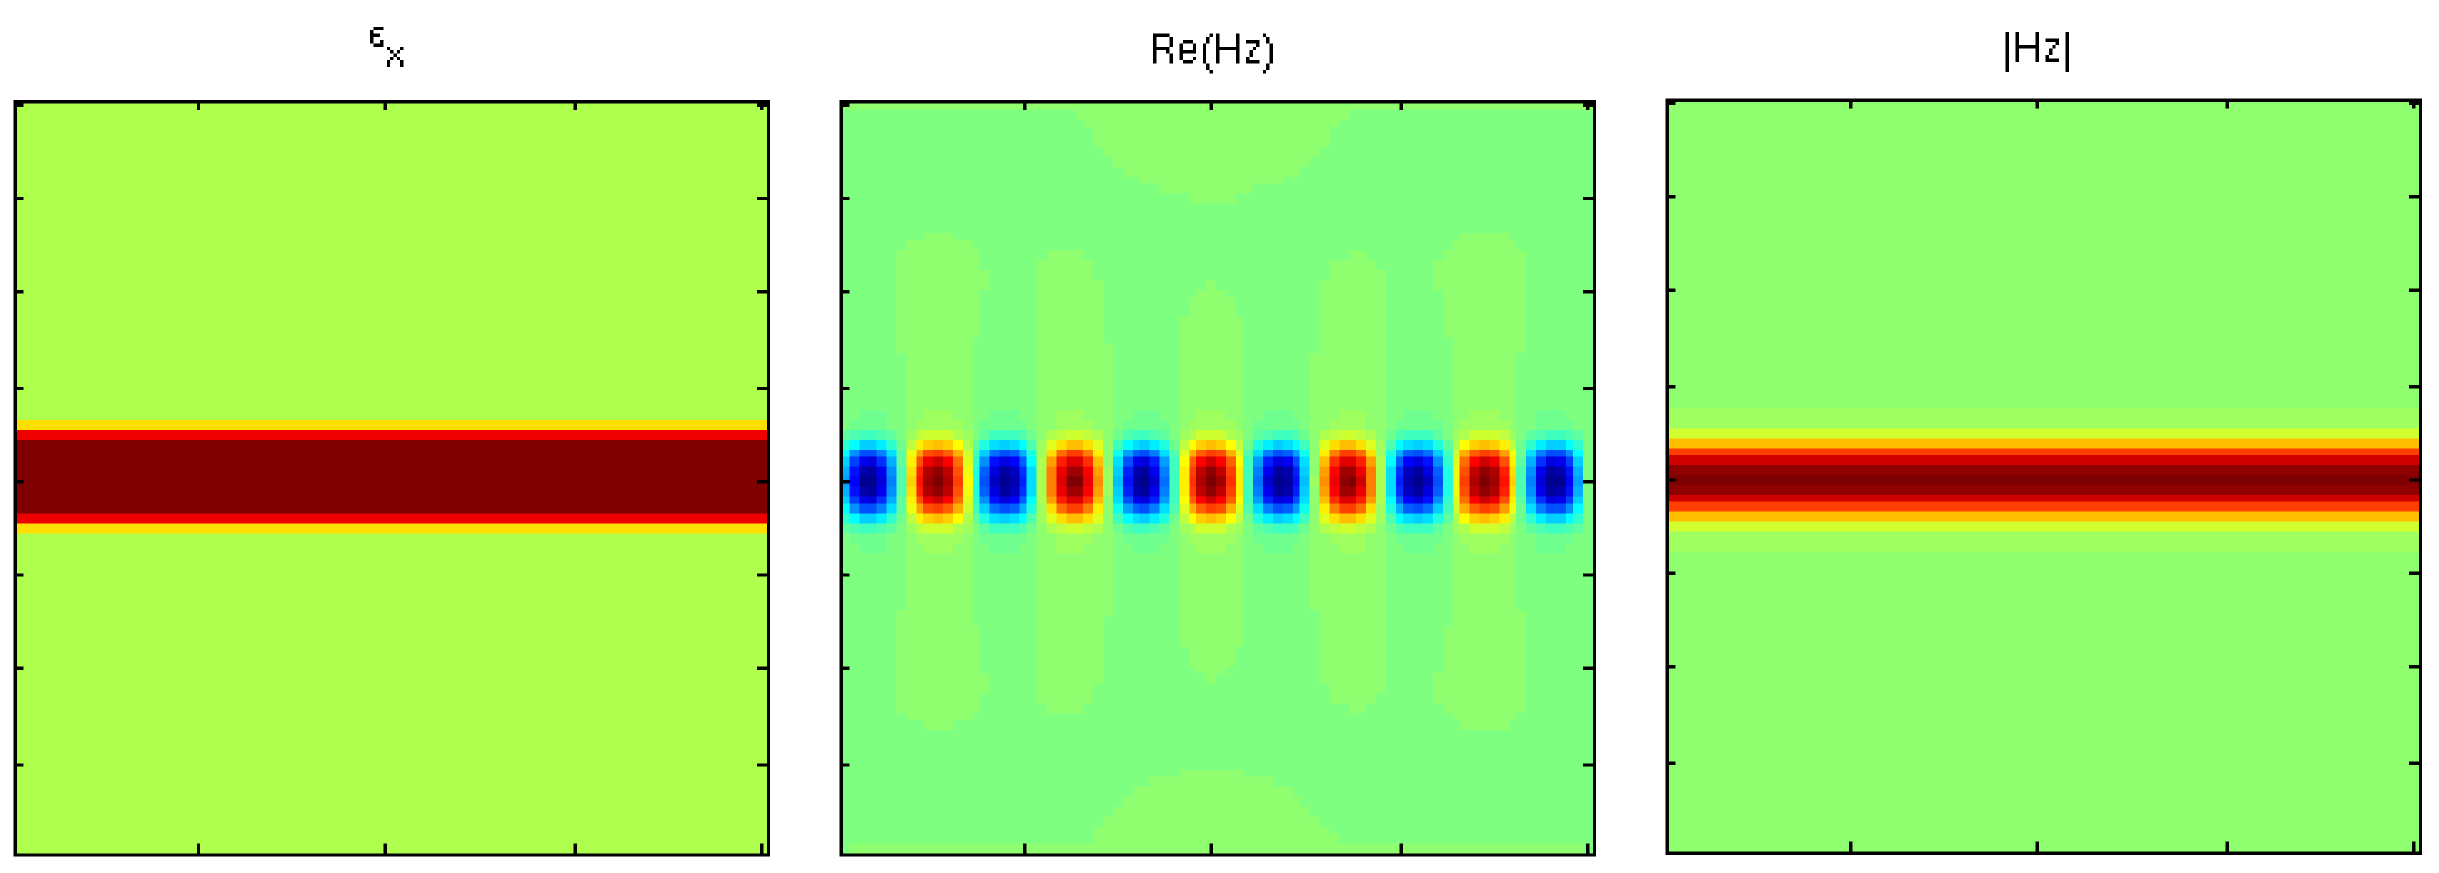
\includegraphics[width=0.8\textwidth]{../figures/waveguide.png}
\end{center}
\item here, $p_0$ is a waveguide structure, and the design objective is a perfect waveguide mode at input and output
\EIT
\newpage

\BIT
\item for general structures and design objectives, this results in a ``soft physics'' field solve
\begin{center}
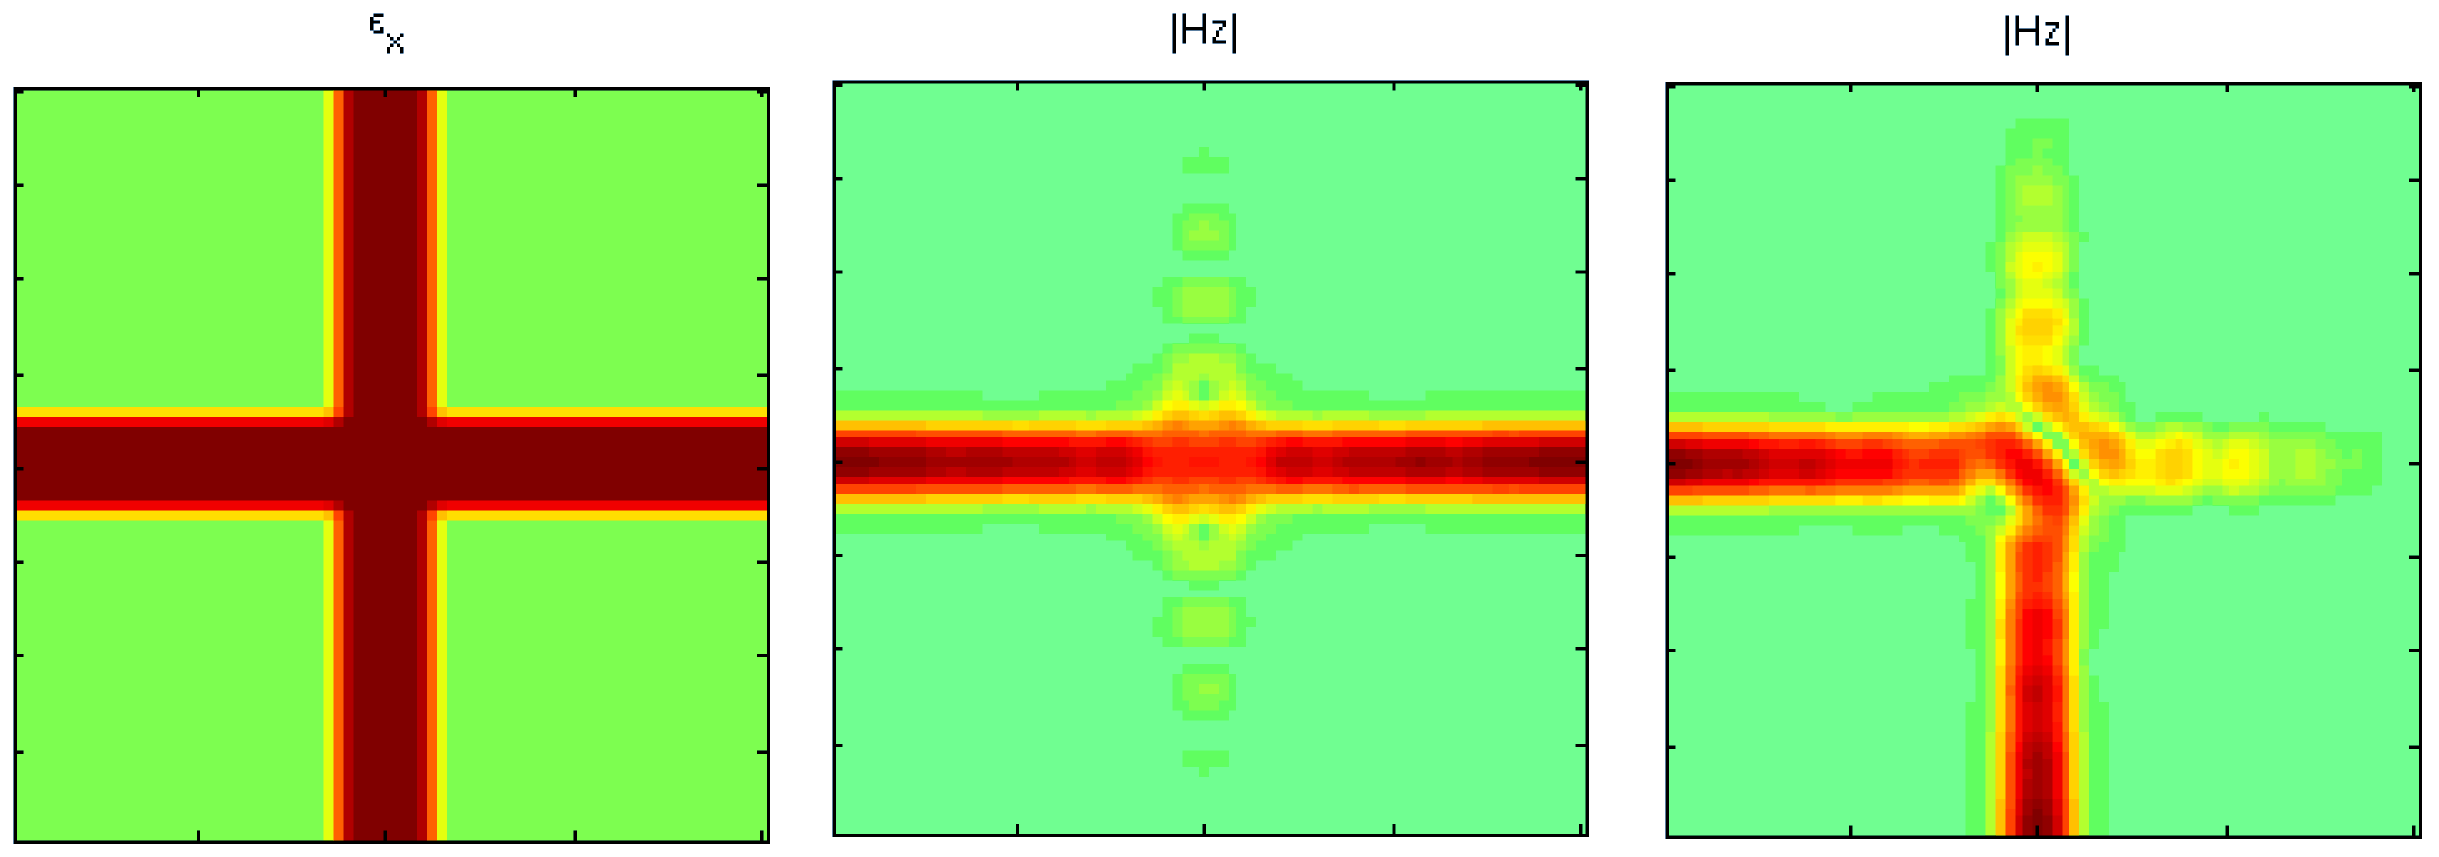
\includegraphics[width=0.8\textwidth]{../figures/crossbar.png}
\end{center}
\item matlab files available at \url{https://github.com/JesseLu/wave-tools}, look for \texttt{em\_bval\_2dte/demo.m}
\EIT
\newpage

\BIT
\item
\EIT


\end{document}
